\documentclass{article}
\usepackage{algorithm}
\usepackage{algpseudocode}
\usepackage{graphicx}
\graphicspath{ {../../images/} }
\usepackage{amssymb}
\usepackage{adjustbox}
\usepackage{placeins}
\usepackage{geometry}
\usepackage{epstopdf}
\geometry{tmargin = 1in}

% Alter some LaTeX defaults for better treatment of figures:
    % See p.105 of "TeX Unbound" for suggested values.
    % See pp. 199-200 of Lamport's "LaTeX" book for details.
    %   General parameters, for ALL pages:
    \renewcommand{\topfraction}{0.9}    % max fraction of floats at top
    \renewcommand{\bottomfraction}{0.8} % max fraction of floats at bottom
    %   Parameters for TEXT pages (not float pages):
    \setcounter{topnumber}{2}
    \setcounter{bottomnumber}{2}
    \setcounter{totalnumber}{4}     % 2 may work better
    \setcounter{dbltopnumber}{2}    % for 2-column pages
    \renewcommand{\dbltopfraction}{0.9} % fit big float above 2-col. text
    \renewcommand{\textfraction}{0.07}  % allow minimal text w. figs
    %   Parameters for FLOAT pages (not text pages):
    \renewcommand{\floatpagefraction}{0.7}  % require fuller float pages
    % N.B.: floatpagefraction MUST be less than topfraction !!
    \renewcommand{\dblfloatpagefraction}{0.7}   % require fuller float pages

\usepackage{color}
\usepackage{xcolor}
\usepackage{listings}
\lstset{
  language= C++,
        % basicstyle=\scriptsize,
        % aboveskip={1.5\baselineskip},
        % columns=fixed,
        showstringspaces=false,
        % extendedchars=false,
        breaklines=true,
        % prebreak = \raisebox{0ex}[0ex][0ex]{\ensuremath{\hookleftarrow}},
        frame=single,
        numbers=left,
        showtabs=false,
        tabsize=3,
        % showspaces=false,
        % showstringspaces=false,
        keywordstyle=\color[HTML]{FF1F54},
        commentstyle=\color[HTML]{008507},
        stringstyle=\color[HTML]{EFAE21},
        numberstyle= \color[HTML]{000000}
}

\renewcommand{\algorithmicforall}{\textbf{for each}}

\begin{document}
\title{Assignment 4: Finite Elements Programming}
%\date{}   
\author{Isaiah Bell} 
\maketitle

\section{Methods}

In this code we solve 2D linear elastic problems over isotropic materials.


\section{Program Design}

The Parallel Unstructured Mesh Infrastructure (PUMI) library was heavily plundered to develop this FE code. A native PUMI mesh was used to represent the discretization of the geometrical model.

The geometrical model definition of the problem is implemented in an embedded Domain Specific Language implemented in C++. Each mesh is generated by operations in this DSL. The shape and size is specified first to create the physical mesh. During the generation of the mesh over the specified geometrical domain, the individual mesh entities are annotated with their corresponding geometrical entities. While PUMI has the capability to import meshes associated with an annotated geometry model, this import capability relies on the output of proprietary software. PUMI provides arbitrary integer tags on mesh elements which are used as keys mapping to boundary conditions. A program is used to generate the mesh for a given geometry was implemented for rectangular domains in memory. These meshes are annotated with integer tags that correspond to geometrical features such as vertices, edges, and faces. Only triangular and quadrilateral element meshes are currently implemented.

The class ElasticAnalysis2D is derived from the base FEAnalysis class and implements
our specific linear elastics definition. This class accepts a PUMI mesh and makes
several assumptions about the mesh structure to determine boundary conditions and
tractions. For memory efficiency the algebraic system is assembled as we iterate over all of the mesh elements. Assembly is simplified by the fact we are using isoparametric elements. The assembly routine loops over each mesh edge and face and attempts to create a stiffness or force contributor. Each mesh entity is visited only once during assembly. The ElasticAnalysis2D calls a method that attempts to make a force 

We extend the apf::Integrator class to implement each stiffness contributor, as well as the discretization of each traction (force contributor). The apf::Integrator class provides way to iterate over integration points for a given integration order.

The PUMI library data structures are used to compute the local contributions, and then values are copied into PETSc structures. There is some effort to optimize these copying operations to occur in bulk for cache efficiencies and in batches of continuous memory locations to minimize cache evictions. These copying routines are implemented in the extraction of the solution displacement vector.


The KSP solver from PETSc was chosen because it had better documentation and examples on its use. The linear system uses PETSc matrices and vectors, allowing for easy choice of a different solver in the future. Default values for the solver were used originally because the example code did not significantly indicate configuration was possible. PETSc architecture allows for changing the parameters of the solver used, or even changing the algorithm completely can be accomplished from a single location in the program in a completely transparent manner to the finite elements code.

\section{Tests}
\subsection{Convergence of Element Types}
\FloatBarrier
We test the convergence of the all of the elements using the same boundary value problem so that direct comparison of convergence is meaningful. The boundary value problem is shown in the figure below. The displacement solution will be cubic, which cannot be exactly represented by our first and second order elements. 


\begin{figure}
    \makebox[\textwidth][c]{\adjustbox{trim= {0.0\width} {0.0\height} {0} {0.0\height}, clip}{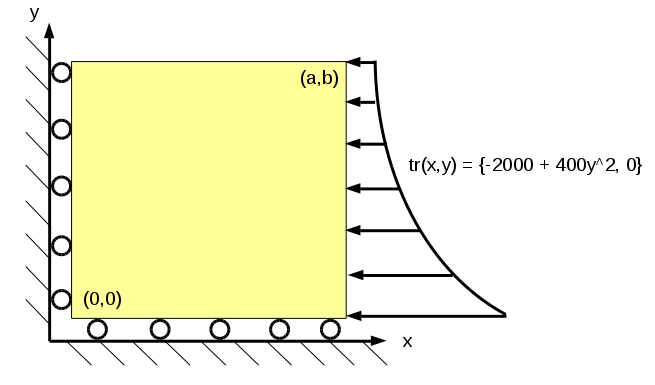
\includegraphics[height = 8cm ]{quadratic_traction}}};
    \caption{Rectangular domain with $a=2$ and $b=2$ units. The left edge has a zero displacement in the x direction boundary condition and a zero displacement in the y direction boundary condition on the bottom edge}
\centering
\end{figure}

\begin{figure}
    \makebox[\textwidth][c]{\adjustbox{trim= {0} {0.25\height} {0} {0.20\height}, clip}{\includegraphics[width = \textwidth ]{convergence_rate}}}
    \caption{Convergence for first and second order finite elements. Substantial inaccuracies that appear as the number of degrees of freedom increase are addressed in the next section.}
\centering
\end{figure}

\pagebreak
%%=================================================================
\subsection{No Displacement Boundary Conditions, No Tractions}
\FloatBarrier

\begin{figure}
    \makebox[\textwidth][c]{\adjustbox{trim= {0.} {0} {0} {0}, clip}{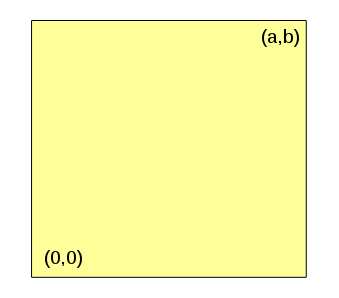
\includegraphics[height = 8cm ]{zero_zero}}};
    \caption{Test boundary value problem: $a = 2$, $b = 2$, $E = 10^8$ and $\nu = 0.35$}
\centering
\end{figure}

With zero constraints and zero tractions, the zero vector is the trivial solution to the linear system. A robust code will properly handle this condition. While other test sections will have a visualization of the displacement solution, the solution to this problem looks exactly the same as the 

\begin{figure}
    \makebox[\textwidth][c]{\adjustbox{trim= {0.1\width} {0.0\height} {0} {0.0\height}, clip}{\includegraphics[width = \textwidth ]{zero_zero_quad_serendipity}}};
    \caption{Linear quadrilateral mesh for a 2 unit by 2 unit rectangular plane shown with displacement scaled by $50,000$ times}
\centering
\end{figure}

\FloatBarrier
%%=================================================================
\subsection{Non Zero Dirichlet Boundary Conditions}
\FloatBarrier

\begin{figure}
    \makebox[\textwidth][c]{\adjustbox{trim= {0.} {0} {0} {0}, clip}{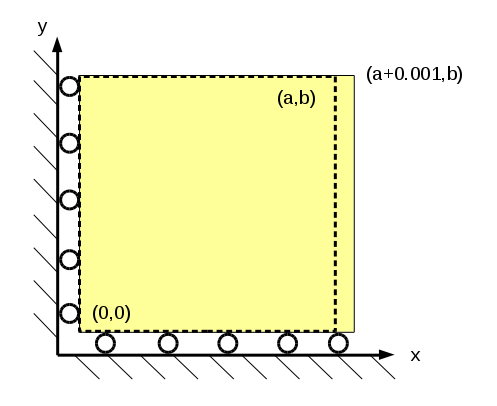
\includegraphics[height = 8cm ]{nonzero_dirichlet}}};
    \caption{Test boundary value problem: $a = 2$, $b = 2$, $E = 10^8$ and $\nu = 0.35$}
\centering
\end{figure}

\FloatBarrier
%%=================================================================
\subsection{Some Boundary Constraints, Constant Traction}
\FloatBarrier

\begin{figure}
    \makebox[\textwidth][c]{\adjustbox{trim= {0.} {0} {0} {0}, clip}{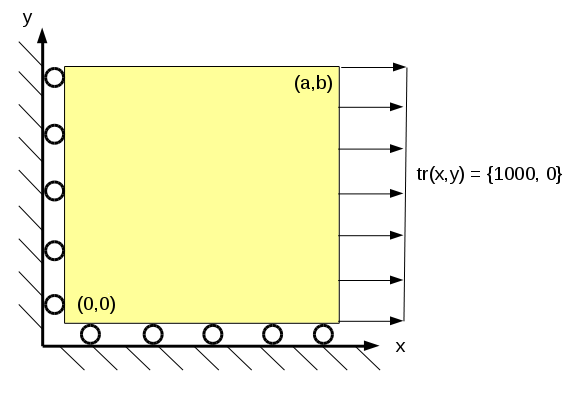
\includegraphics[height = 8cm ]{linear_traction}}};
    \caption{Test boundary value problem: $a = 2$, $b = 2$, $E = 10^8$ and $\nu = 0.35$}
\centering
\end{figure}


\begin{figure}
    \makebox[\textwidth][c]{\adjustbox{trim= {0.1\width} {0.0\height} {0} {0.0\height}, clip}{\includegraphics[width = \textwidth ]{constant_traction_linear_quad}}};
    \caption{Linear quadrilateral mesh for a 2 unit by 2 unit rectangular plane shown with displacement scaled by $50,000$ times}
\centering
\end{figure}

\begin{figure}
    \makebox[\textwidth][c]{\adjustbox{trim= {0.1\width} {0.0\height} {0} {0.0\height}, clip}{\includegraphics[width = \textwidth ]{constant_traction_linear_tri}}};
    \caption{Linear triangle mesh for a 2 unit by 2 unit rectangular plane shown with displacement scaled by $50,000$ times}
\centering
\end{figure}

\begin{figure}
    \makebox[\textwidth][c]{\adjustbox{trim= {0.1\width} {0.0\height} {0} {0.0\height}, clip}{\includegraphics[width = \textwidth ]{constant_traction_quad_quad}}};
    \caption{Quadratic quadrilateral mesh for a 2 unit by 1 unit rectangular plane shown with displacement scaled by $50,000$ times}
\centering
\end{figure}


\begin{figure}
    \makebox[\textwidth][c]{\adjustbox{trim= {0.1\width} {0.0\height} {0} {0.0\height}, clip}{\includegraphics[width = \textwidth ]{constant_traction_serendipity_quad}}};
    \caption{Serendipity mesh for a 2 unit by 2 unit rectangular plane shown with displacement scaled by $50,000$ times}
\centering
\end{figure}

\FloatBarrier
%%=================================================================
\subsection{Some Boundary Constraints,  Quadratic Traction}
\FloatBarrier

\begin{figure}
    \makebox[\textwidth][c]{\adjustbox{trim= {0.} {0} {0} {0}, clip}{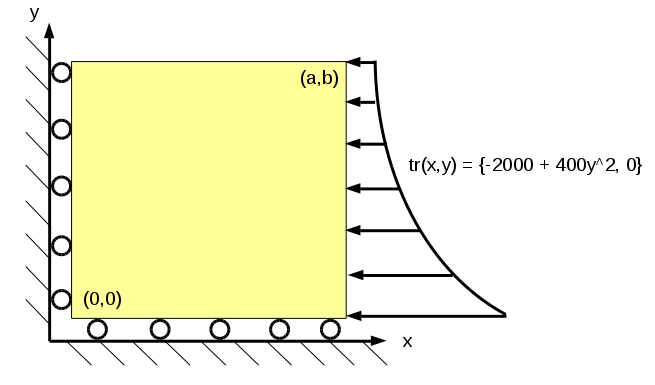
\includegraphics[height = 8cm ]{quadratic_traction}}};
    \caption{Test boundary value problem: $a = 2$, $b = 2$, $E = 10^8$ and $\nu = 0.35$}
\centering
\end{figure}

\begin{figure}
    \makebox[\textwidth][c]{\adjustbox{trim= {0.1\width} {0.0\height} {0} {0.0\height}, clip}{\includegraphics[width = \textwidth ]{quad_traction_linear_quad}}};
    \caption{Linear quadrilateral mesh for a 2 unit by 2 unit rectangular plane shown with displacement scaled by $50,000$ times}
\centering
\end{figure}

\begin{figure}
    \makebox[\textwidth][c]{\adjustbox{trim= {0.1\width} {0.0\height} {0} {0.0\height}, clip}{\includegraphics[width = \textwidth ]{quad_traction_linear_tri}}};
    \caption{Linear triangle mesh for a 2 unit by 2 unit rectangular plane shown with displacement scaled by $50,000$ times}
\centering
\end{figure}

\begin{figure}
    \makebox[\textwidth][c]{\adjustbox{trim= {0.1\width} {0.0\height} {0} {0.0\height}, clip}{\includegraphics[width = \textwidth ]{quad_traction_quad_quad}}};
    \caption{Quadratic quadrilateral mesh for a 2 unit by 1 unit rectangular plane shown with displacement scaled by $50,000$ times}
\centering
\end{figure}


\begin{figure}
    \makebox[\textwidth][c]{\adjustbox{trim= {0.1\width} {0.0\height} {0} {0.0\height}, clip}{\includegraphics[width = \textwidth ]{quad_traction_serendipity_quad}}};
    \caption{Serendipity mesh for a 2 unit by 2 unit rectangular plane shown with displacement scaled by $50,000$ times}
\centering
\end{figure}

\FloatBarrier
%%=================================================================
\subsection{Some Boundary Constraints, Constant Body Force}
\FloatBarrier

\begin{figure}
    \makebox[\textwidth][c]{\adjustbox{trim= {0.} {0} {0} {0}, clip}{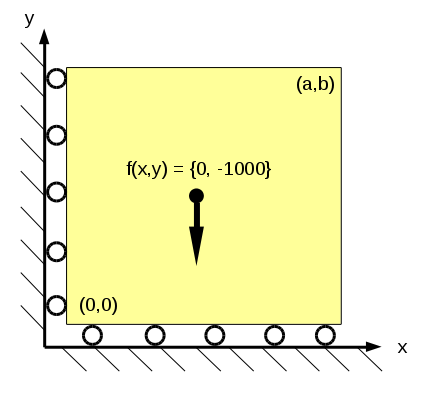
\includegraphics[height = 8cm ]{constant_body}}};
    \caption{Test boundary value problem: $a = 2$, $b = 1$, $E = 10^8$ and $\nu = 0.35$}
\centering
\end{figure}

\begin{figure}
    \makebox[\textwidth][c]{\adjustbox{trim= {0.1\width} {0.10\height} {0} {0.25\height}, clip}{\includegraphics[width = \textwidth ]{gravity_linear_quad}}};
    \caption{Linear quadrilateral mesh for a 2 unit by 1 unit rectangular plane shown with displacement scaled by $50,000$ times}
\centering
\end{figure}

\begin{figure}
    \makebox[\textwidth][c]{\adjustbox{trim= {0.1\width} {0.10\height} {0} {0.25\height}, clip}{\includegraphics[width = \textwidth ]{gravity_linear_tri}}};
    \caption{Linear triangle mesh for a 2 unit by 1 unit rectangular plane shown with displacement scaled by $50,000$ times}
\centering
\end{figure}

\begin{figure}
    \makebox[\textwidth][c]{\adjustbox{trim= {0.1\width} {0.10\height} {0} {0.25\height}, clip}{\includegraphics[width = \textwidth ]{gravity_quadratic_quad}}};
    \caption{Quadratic quadrilateral mesh for a 2 unit by 1 unit rectangular plane shown with displacement scaled by $50,000$ times}
\centering
\end{figure}


% \begin{figure}
%     \makebox[\textwidth][c]{\adjustbox{trim= {0.1\width} {0.10\height} {0} {0.25\height}, clip}{\includegraphics[width = \textwidth ]{gravity_linear_quad}}};
%     \caption{Quadratic triangle mesh for a 2 unit by 1 unit rectangular plane shown with displacement scaled by $50,000$ times}
% \centering
% \end{figure}

\begin{figure}
    \makebox[\textwidth][c]{\adjustbox{trim= {0.1\width} {0.10\height} {0} {0.25\height}, clip}{\includegraphics[width = \textwidth ]{gravity_serendipity_quad}}};
    \caption{Serendipity mesh for a 2 unit by 1 unit rectangular plane shown with displacement scaled by $50,000$ times}
\centering
\end{figure}


\FloatBarrier

%%=================================================================
\subsection{Some Boundary Constraints, Linear Body Force}
\FloatBarrier

\begin{figure}
    \makebox[\textwidth][c]{\adjustbox{trim= {0.} {0} {0} {0}, clip}{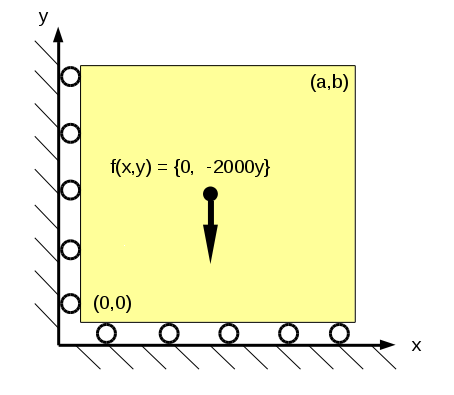
\includegraphics[height = 8cm ]{linear_body}}};
    \caption{Test boundary value problem: $a = 2$, $b = 2$, $E = 10^8$ and $\nu = 0.35$}
\centering
\end{figure}

\begin{figure}
    \makebox[\textwidth][c]{\adjustbox{trim= {0.1\width} {0.0\height} {0} {0.0\height}, clip}{\includegraphics[width = \textwidth ]{linear_body_linear_quad}}};
    \caption{Linear quadrilateral mesh for a 2 unit by 2 unit rectangular plane shown with displacement scaled by $50,000$ times}
\centering
\end{figure}

\begin{figure}
    \makebox[\textwidth][c]{\adjustbox{trim= {0.1\width} {0.0\height} {0} {0.0\height}, clip}{\includegraphics[width = \textwidth ]{linear_body_linear_tri}}};
    \caption{Linear triangle mesh for a 2 unit by 2 unit rectangular plane shown with displacement scaled by $50,000$ times}
\centering
\end{figure}

\begin{figure}
    \makebox[\textwidth][c]{\adjustbox{trim= {0.1\width} {0.0\height} {0} {0.0\height}, clip}{\includegraphics[width = \textwidth ]{linear_body_quad_quad}}};
    \caption{Quadratic quadrilateral mesh for a 2 unit by 1 unit rectangular plane shown with displacement scaled by $50,000$ times}
\centering
\end{figure}


\begin{figure}
    \makebox[\textwidth][c]{\adjustbox{trim= {0.1\width} {0.0\height} {0} {0.0\height}, clip}{\includegraphics[width = \textwidth ]{linear_body_serendipity_quad}}};
    \caption{Serendipity mesh for a 2 unit by 2 unit rectangular plane shown with displacement scaled by $50,000$ times}
\centering
\end{figure}


\FloatBarrier

\section{Notable Bugs}

\FloatBarrier

\begin{figure}
    \makebox[\textwidth][c]{\adjustbox{trim= {0} {0.2\height} {0} {0.15\height}, clip}{\includegraphics[width = 0.8\textwidth ]{smaller_h_constant_force}}};
    \caption{Convergence of meshes of same geometrical problem with different types of mesh elements. $E = 8*10^8$ and $\nu = 0.35$}
\centering
\end{figure}
We change the size of the domain of the boundary value problem to detect any type of rounding errors or loss of precision from underflow. Using a domain that is an order of magnitude larger that the first problem, the error with the strain energy does not change noticeably.
\begin{figure}
    \makebox[\textwidth][c]{\adjustbox{trim= {0} {0.2\height} {0} {0.15\height}, clip}{\includegraphics[width = 0.8\textwidth ]{smaller_h_constant_force_20x20}}};
    \caption{Convergence of meshes of same geometrical problem with different types of mesh elements. $E = 8*10^8$ and $\nu = 0.35$}
\centering
\end{figure}


\begin{figure}
    \makebox[\textwidth][c]{\adjustbox{trim= {0} {0.2\height} {0} {0.15\height}, clip}{\includegraphics[width = 0.8\textwidth ]{difference_between_10_80_linear_tri_gravity}}};
    \caption{Difference in deformation solution between a 10x10 mesh and a 80x80 mesh for linear triangle elements. $E = 8*10^8$ and $\nu = 0.35$}
\centering
\end{figure}
\FloatBarrier
We check to see if this could be an issue with the chosen solver finding a close enough solution to the systems of equations. We are using an inexact solver, so this scenario is plausible. Plotting the strain energy against the degrees of freedom will reveal any dependence on solver inaccuracies.
\FloatBarrier
\begin{figure}
    \makebox[\textwidth][c]{\adjustbox{trim= {0} {0.2\height} {0} {0.15\height}, clip}{\includegraphics[width = 0.8\textwidth ]{error_vs_dofs}}};
    \caption{Strain energy plotted vs degrees of freedom in the linear system passed to the solver which has fixed degrees of freedom from boundary constraints already reduced}
\centering
\end{figure}
\FloatBarrier
From the figure we see two different behaviors for different mesh elements. The quadrilateral elements all show similar degradation in the accuracy of the solution at around 15 thousand degrees of freedom. For triangular elements the loss in accuracy does not appear to have a common break point. This indicates that there is a separate bug with the implementation of triangular elements. Implementing the third order Lagrange shape functions would help test this hypothesis. Right now there are only two data points for the behavior of triangular elements, which makes pattern fitting more difficult. Checking the norm of the solution produced by the solver $||Kd - F||$ would also give more information about potential implementation errors or misuse of PETSc solvers.


\FloatBarrier
\section{Pseudo code}

Not completed

% \begin{algorithm}
% \begin{algorithmic}

% \Procedure{Foo}{bar}
%     \State Foo
% \EndProcedure

% \end{algorithmic}
% \end{algorithm}

% \begin{algorithm}
% \begin{algorithmic}

% \Procedure{IntegrateStiffness}{element, weight, dV}
%     \State n\_local\_dofs $\gets$ NDIM $*$ countElementNodes(element) \Comment{2} 
%     \State K\_element $\gets$ Matrix< n\_local\_dofs, n\_local\_dofs >
%     \ForAll{integration\_point \textbf{on} element}
%         \State gradShape $\gets$ getShapeGradient(integration\_point)
%         \Comment Construct
%         \ForAll{node \textbf{in} element}
%             \State B[node\_index] $\gets$ $ \left[  \right]$
%         \EndFor
%     \EndFor
% \EndProcedure

% \end{algorithmic}
% \end{algorithm}



% \begin{figure}
%     \makebox[\textwidth][c]{\adjustbox{trim= {0.15\width} {0} {0.15\width} {0}, clip}{\includegraphics[width = \textwidth ]{part1_pre_migr}}};
%     \caption{Partition 1 surface before region migration}
% \centering


\section{Source Code Listings}

\lstset{linewidth = 16cm, xrightmargin = 0cm}
\lstlistoflistings
%includes
\lstinputlisting[caption = {Algebraic System container class}]{../inc/AlgebraicSystem.h}
\lstinputlisting[caption = {Elastic Analysis Class}]{../inc/ElasticAnalysis2D.h}
\lstinputlisting[caption = {Abstract Base FE Analysis class}]{../inc/FEAnalysis.h}
\lstinputlisting[caption = {Force Contributor}]{../inc/ForceContributor2D.h}
\lstinputlisting[caption = {Mesh Builder helper class}]{../inc/MeshBuilder.h}
\lstinputlisting[caption = {Adjacency reordering routine}]{../inc/MeshAdjReorder.h}
\lstinputlisting[caption = {Stiffness Constributor}]{../inc/StiffnessContributor2D.h}
\lstinputlisting[caption = {Recover Secondary Variables}]{../inc/RecoverAtIntegrationPoints.h}

%sources
\lstinputlisting[caption = {Algebraic System implementation}]{../src/AlgebraicSystem.cc}
\lstinputlisting[caption = {Elastic Analysis implementation}]{../src/ElasticAnalysis2D.cc}
\lstinputlisting[caption = {Force Contributor implementation}]{../src/ForceContributor2D.cc}

\lstinputlisting[caption = {Stiffness contributor implementation}]{../src/StiffnessContributor2D.cc}
\lstinputlisting[caption = {Geometry Mapping Implementation}]{../src/GeometryMappings.cc}
\lstinputlisting[caption = {Mesh Adjacency reordering implementation}]{../src/MeshAdjReorder.cc}
\lstinputlisting[caption = {Mesh builder scripts}]{../src/MeshBuilder.cc}

%tests
\lstinputlisting[caption = {Test Driver}]{../src/mpi_and_petsc_gtest_main.cc}
%Mesh builder unittests are all empty right now and probably wont meaningfully change
%\lstinputlisting[caption = {Mesh builder unittests}]{../src/MeshBuilder_unittest.cc}
\lstinputlisting[caption = {Measures convergence of mesh elements}]{../src/Convergence_test.cc}
\lstinputlisting[caption = {Abstract common testing setup code}]{../inc/TestingUtilityFunctions.h}
\lstinputlisting[caption = {Algebraic System tests}]{../src/AlgebraicSystem_unittest.cc}
\lstinputlisting[caption = {Test node mapping functions}]{../src/ShapeFunctionOrdering_unittest.cc}
\lstinputlisting[caption = {Test mesh generation scripts}]{../src/SimpleRectMesh_unittest.cc}
\lstinputlisting[caption = {Geometry Mapping tests}]{../src/GeometryMappings_unittest.cc}

%build files
\lstinputlisting[caption = {configuration file}]{../config.mk}
\lstinputlisting[caption = {Makefile}]{../Makefile}
\lstinputlisting[caption = {Travis CI}] {../../.travis.yml}


\end{document}
